\documentclass{article}

\usepackage{graphicx}
\usepackage{multirow}
\usepackage{color}
\usepackage[citecolor=black,linkcolor=black,urlcolor=blue,colorlinks=true]{hyperref}
\title{Note: Machine Learning Introduction}
\author{Sun Zhao}

\begin{document}
\maketitle
\newpage

\section{Definition of Machine Learning}
I've heard of lots of famous machine learning algorithm like SVM, collaborate recommending, LSH and applications like google machine translation. Those algorithms and applications make me believe that machine learning is powerful and useful. So, what is machine learning? Arthur Samuel said that Machine learning was a field of study that gave computer the ability to learn without being explicitly programmed. He wrote a checker's playing program watching tens of thousands games to learn what tends to be good positions and what tends to be bad positions. And finally, the program was much better at playing games than Arthur Samuel himself. Wow, this is really a remarkable point showing the learning ability of machine. Tom Mitchell(1998) defined machine learning problem as: A computer program is said to learn from experience E with respect to some task T and some performance measure P, if its performance on T, as measured by P, improves with experience E. For example, we have a email program watching which emails are marked as spam or non-spam, and the program bases on that to learn how to better filter spam. In the case, classifying emails as spam or not spam is the task of T, watching emails' labels is the experience of E, and the number of emails correctly classified as spam or not spam is the performance measure of P. I think this definition is much more format than previous one, however, one sided. Because in the case of unsupervised learning, no "right answers" are provided, so the experience of E and performance measure P are obscure. In my opinion, Arthur Samuel's definition reveals the intrinsic of machine learning.

\section{Supervised Learning}
Example 1: Look at Fig. \ref{example1_of_supervised_learning}, it shows the relationship between price and area of a house. The red cross points are the so called "right answers" also the given data set. The machine learning problem is if we have another new size of a house area, what's the expected price of this house? Naturally, we can use a curve or a straight line(also a special curve) to describe the relationship with all given pointers. So questions are what is the cost function of this model and how to optimize it? Now, I know the regression model can solve them all.\\
Example 2: Look at Fig. \ref{example2_of_supervised_learning}, it shows the relationship between tumor size and tumor property(malignant or benign). Blue cross pointers are tumors turning out to be benign and red cross pointers are that turning out to be malignant. The machine learning problem is if we are given a new tumor size, can we predict whether it is malignant or benign. Now, I know this is a classification problem.\\
Summary: A supervised learning algorithm analyzes the training data(the "right answers") and produces an inferred function. If the output of the inferred function is continuous, then it becomes a regression function, otherwise a classification function. As a result, example 1 is a regression problem and example 2 is a classification problem.
\begin{figure}[ht]
  \centering
  % Requires \usepackage{graphicx}
  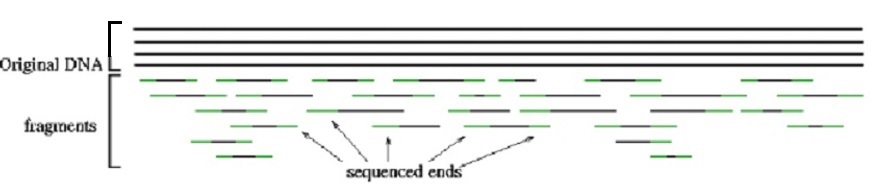
\includegraphics[width=10cm]{Figure1.jpg}\\
  \caption{}\label{example1_of_supervised_learning}
\end{figure}
\begin{figure}[ht]
  \centering
  % Requires \usepackage{graphicx}
  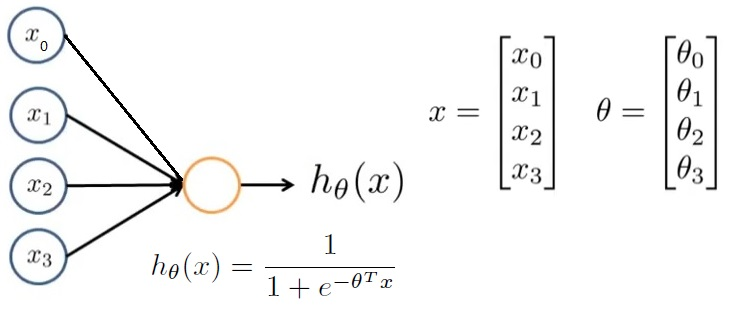
\includegraphics[width=10cm]{Figure2.jpg}\\
  \caption{}\label{example2_of_supervised_learning}
\end{figure}
\section{Unsupervised Learning}
Different from supervised learning, the given data set for unsupervised learning has no labels. Unsupervised learning algorithms are trying to find structure information on the data set. Google news(news.google.com) is a good application of unsupervised learning. It crawls millions of news from web sites, and display them in different topic groups for easy reading. Teacher showed a very interesting and famous problem called cocktail problem at the end of the class. Cocktail problem describe a occasion that two speakers talks simultaneously to two microphones, and because the distance between the microphone and speakers are different, the output of each microphone contains two concurrent sounds(one is light and the other one is clearly loud). Unsupervised learning algorithms will produce two clear sound from the two light and clear mixed sounds. And such a task can be done with one line of code! It is really cool that one line of code can accomplish such a complex problem. Teacher also recommended machine learning programming langues like Octave and Matlab. Without these powerful programming langues, the cocktail problem cannot be solved within one line of code.

\section{Summary}
Machine learning algorithm consists of two categories algorithms: supervised learning and unsupervised learning algorithms. Supervised learning algorithm finds an inferred function to predict values on labeled data set. Unsupervised learning algorithms finds structures on data set without labels. We should use Octave or Matlab like programming languages other than C++ or Java.
\end{document}
